\begin{frame}[plain,c]
  \begin{center}
    \Huge Model ARX
  \end{center}
\end{frame}

\begin{frame}
  \frametitle{Model ARX- zasada działania}
  \begin{block}{Założenia:}
    \begin{itemize}
      \item dobranie wejść modelu przy pomocy współczynnika korelacji,
        \begin{itemize}
          \item weryfikacja skrośna wszystkich zestawów danych,
          \item dobranie na podstawie jednego zestawu, 
        \end{itemize}
      \item dobranie stopni wielomianów modelu przy pomocy algorytmu genetycznego (ga),
      \item wyznaczenie parametrów modelu ARX wykorzystując MNK przy wcześniejszym ustaleniu liczby wejść.
    \end{itemize}
  \end{block}

  \begin{block}{Dla przychodzącego zestawu wejść:}
    \begin{itemize}
      \item wykorzystanie danych historycznych,
      \item przemnożenie przez wektor wyznaczonych parametrów. 
    \end{itemize}
  \end{block}
\end{frame}

\begin{frame}
  \frametitle{Model ARX - przygotowanie danych i uczenie modelu}
  \begin{block}{Operacja wykonywane na danych uczących}
    \begin{itemize}
      \item wyznaczenie sygnałów wejściowych na podstawie współczynnika korelacji,
      \item interpolacja/usunięcie próbek brakujących/nadmiarowych,
      \item podział danych na zestawy,
      \begin{itemize}
        \item uczący (z. 1 oraz z. 2),
        \item weryfikujący (z. 3 oraz z. 4).
      \end{itemize}
    \end{itemize}
  \end{block}

  \begin{block}{Proces uczenia modelu:}
    \begin{itemize}
      \item dobranie współczynnika minimalnej korelacji,
      \item na podstawie wyznaczonych wejść opracowanie modelu wstępnego arx z danych uczących,
      \item sprawdzenie poprawności modelu na podstawie zestawu weryfikującego.
    \end{itemize}
  \end{block}
\end{frame}



\begin{frame}
  \frametitle{Działanie modelu ARX dla sygnału LT01}
  \begin{figure}[H]
    \centering
    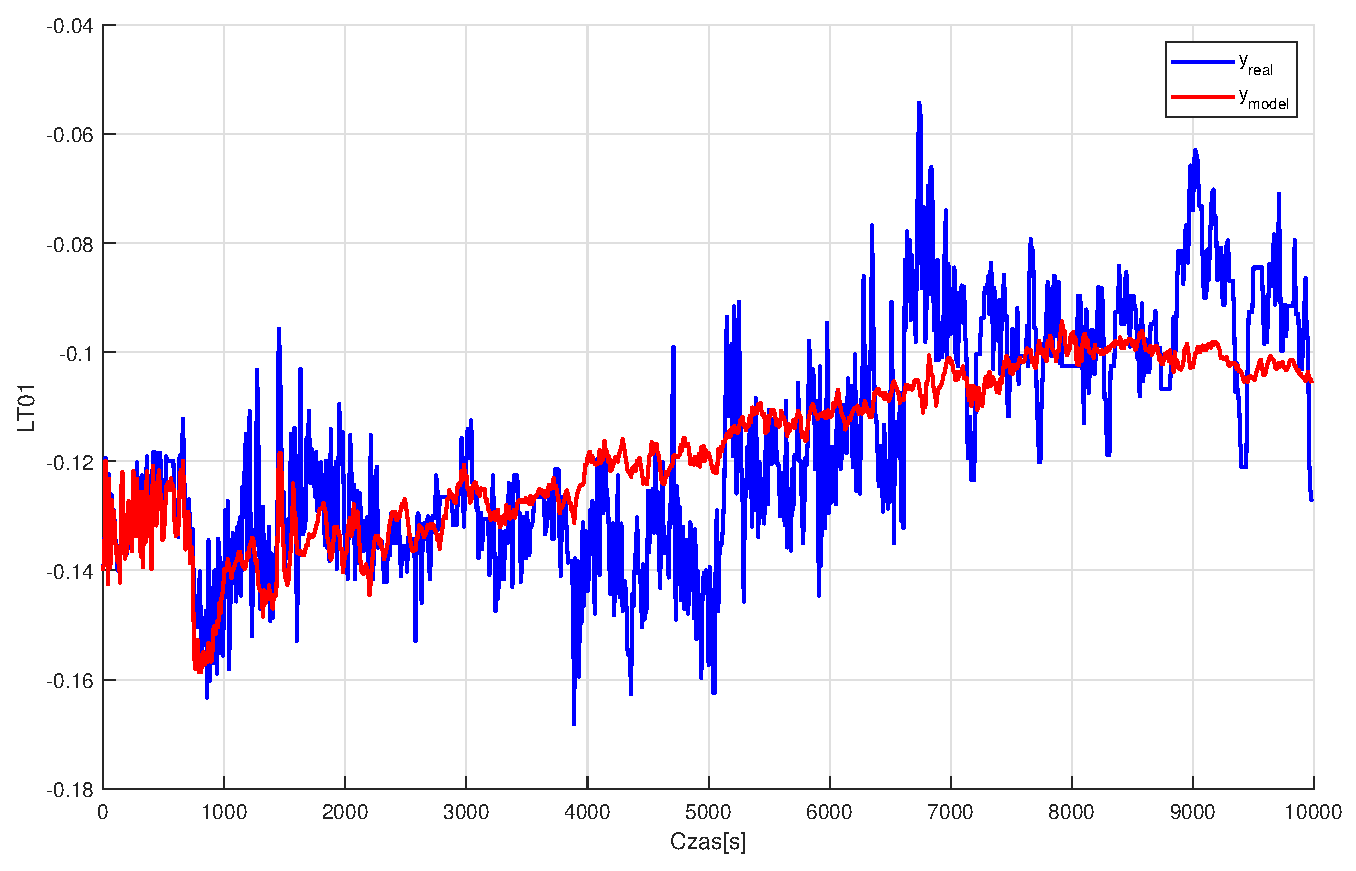
\includegraphics[width=0.75\linewidth,keepaspectratio]{results_matlab/LT01_1.eps}
    \caption{Porównanie działania modelu ARX z danymi uczącymi (z. 1)}
    \label{fig:test}
    \end{figure}
\end{frame}

\addtocounter{framenumber}{-1}
\begin{frame}
  \frametitle{Działanie modelu ARX dla sygnału LT01}
  \begin{figure}[H]
    \centering
    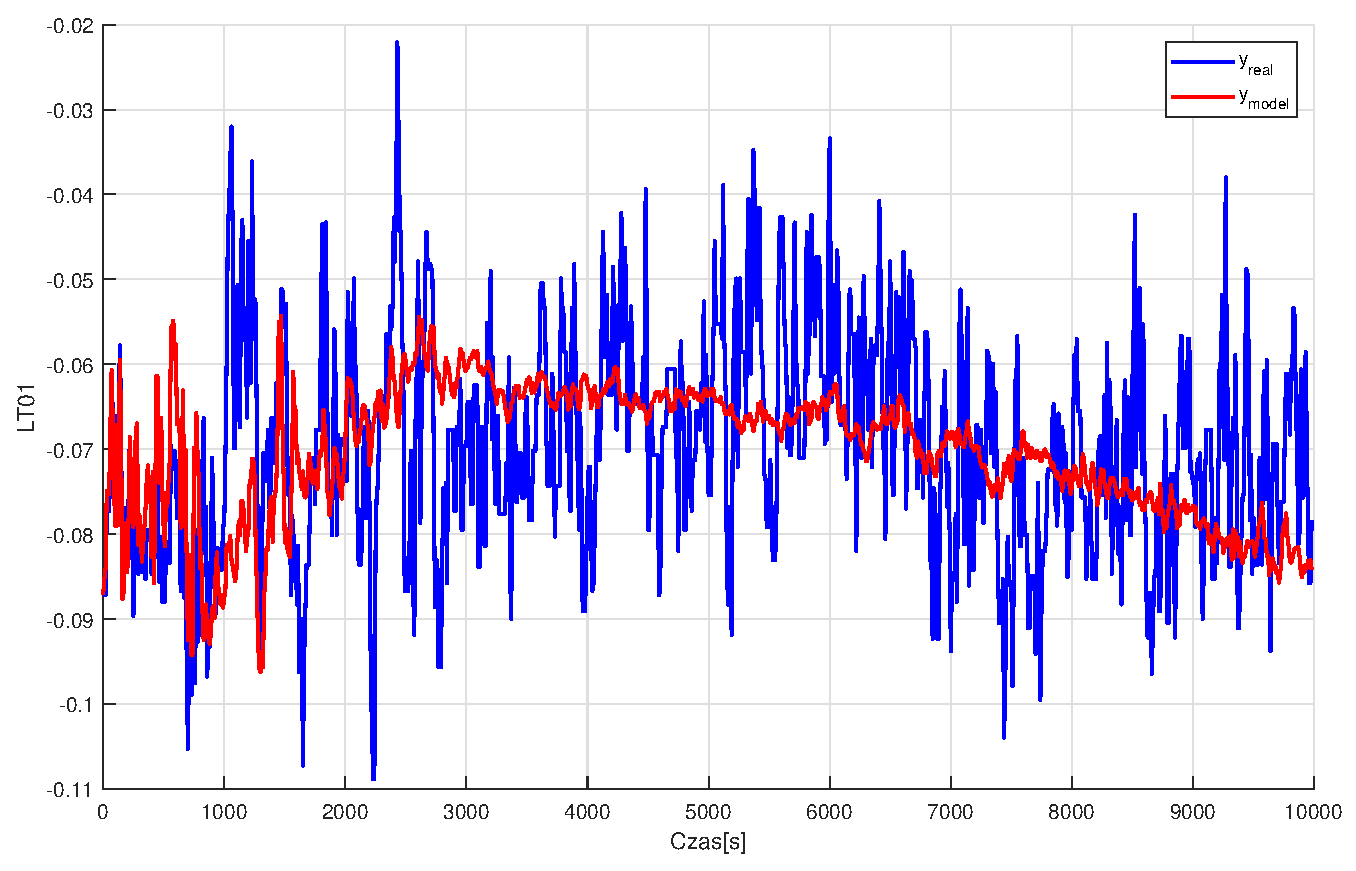
\includegraphics[width=0.75\linewidth,keepaspectratio]{results_matlab/LT01_2.eps}
    \caption{Porównanie działania modelu ARX z danymi uczącymi (z. 2)}
    \label{fig:test}
    \end{figure}
\end{frame}

\addtocounter{framenumber}{-1}
\begin{frame}
  \frametitle{Działanie modelu ARX dla sygnału LT01}
  \begin{figure}[H]
    \centering
    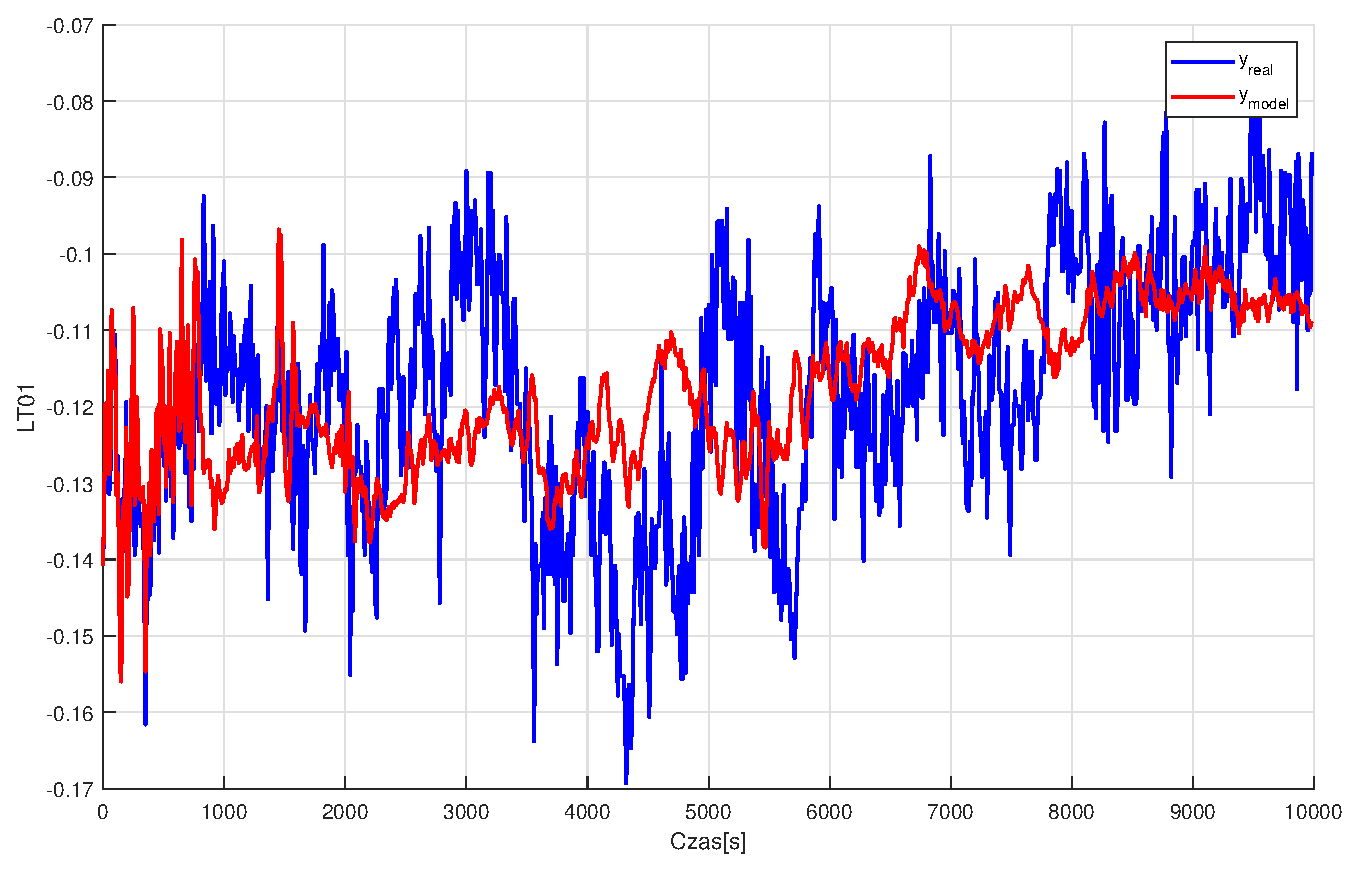
\includegraphics[width=0.75\linewidth,keepaspectratio]{results_matlab/LT01_3.eps}
    \caption{Porównanie działania modelu ARX z danymi weryfikacyjnymi (z. 3)}
    \label{fig:test}
    \end{figure}
\end{frame}

\addtocounter{framenumber}{-1}
\begin{frame}
  \frametitle{Działanie modelu ARX dla sygnału LT01}
  \begin{figure}[H]
    \centering
    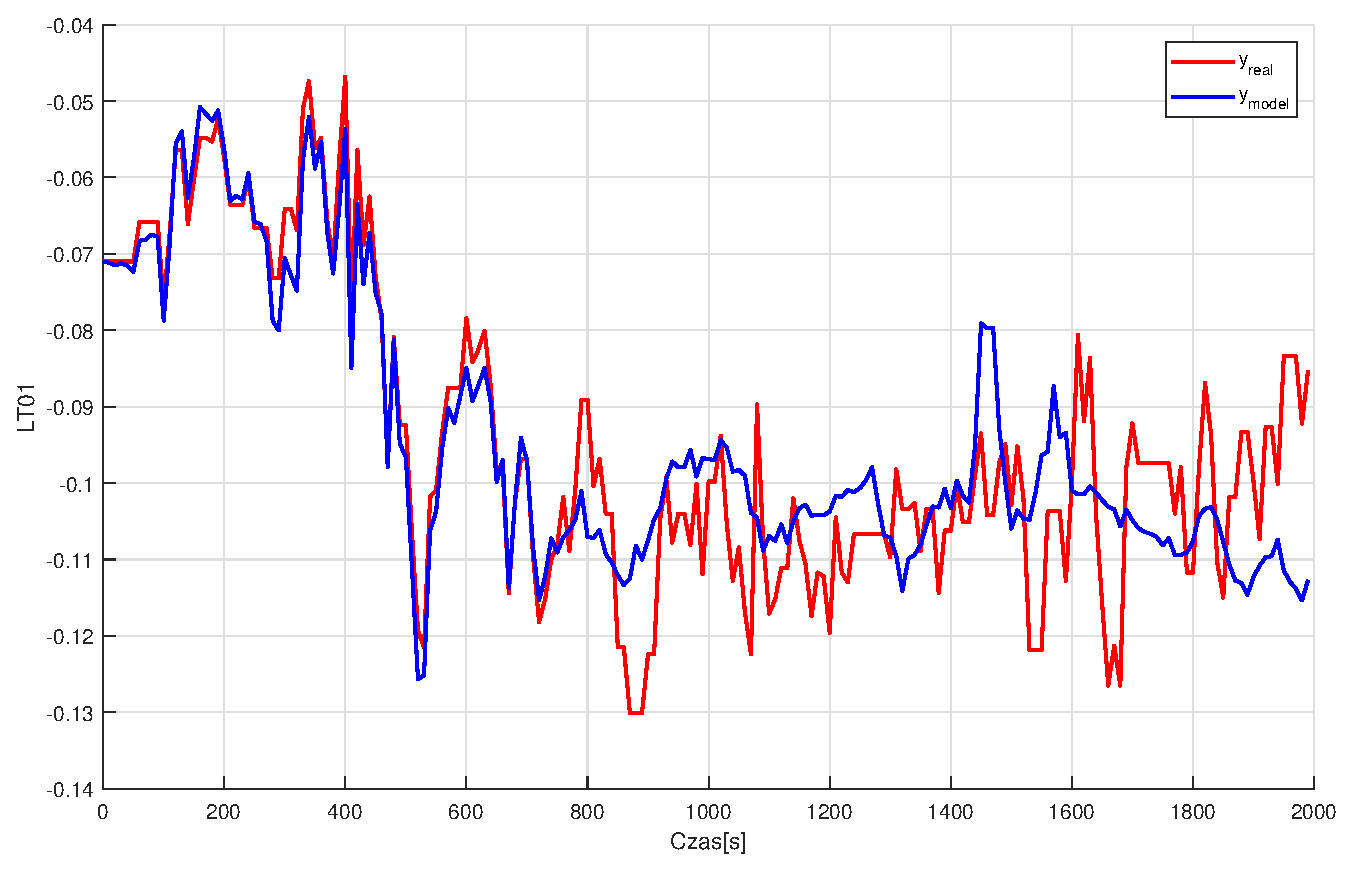
\includegraphics[width=0.75\linewidth,keepaspectratio]{results_matlab/LT01_4.eps}
    \caption{Porównanie działania modelu ARX z danymi weryfikacyjnymi (z. 4)}
    \label{fig:test}
    \end{figure}
\end{frame}

\begin{frame}
  \frametitle{Działanie modelu ARX dla sygnału DP}
  \begin{figure}[H]
    \centering
    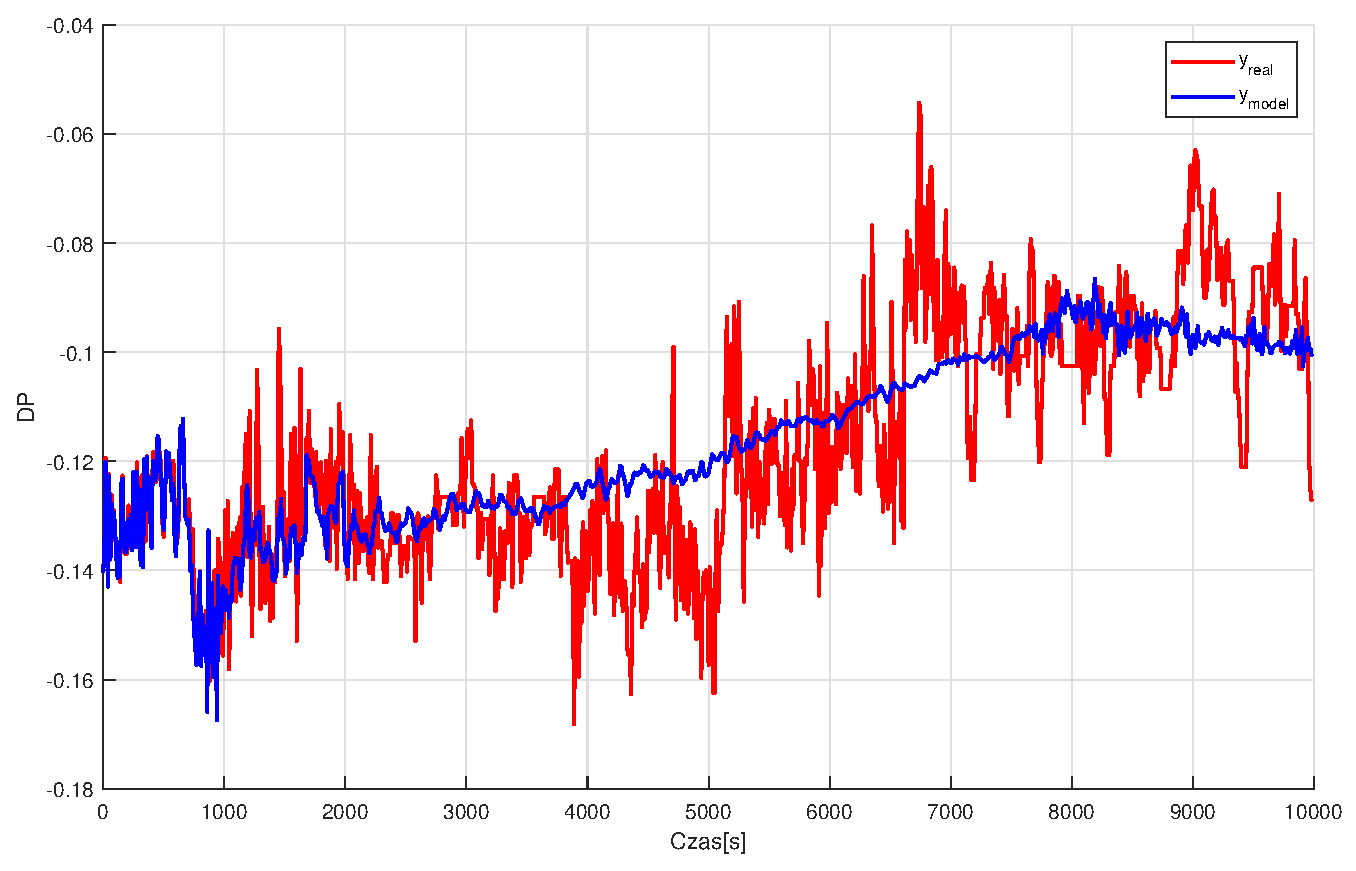
\includegraphics[width=0.75\linewidth,keepaspectratio]{results_matlab/DP_1.eps}
    \caption{Porównanie działania modelu ARX z danymi uczącymi (z. 1)}
    \label{fig:test}
    \end{figure}
\end{frame}

\addtocounter{framenumber}{-1}
\begin{frame}
  \frametitle{Działanie modelu ARX dla sygnału DP}
  \begin{figure}[H]
    \centering
    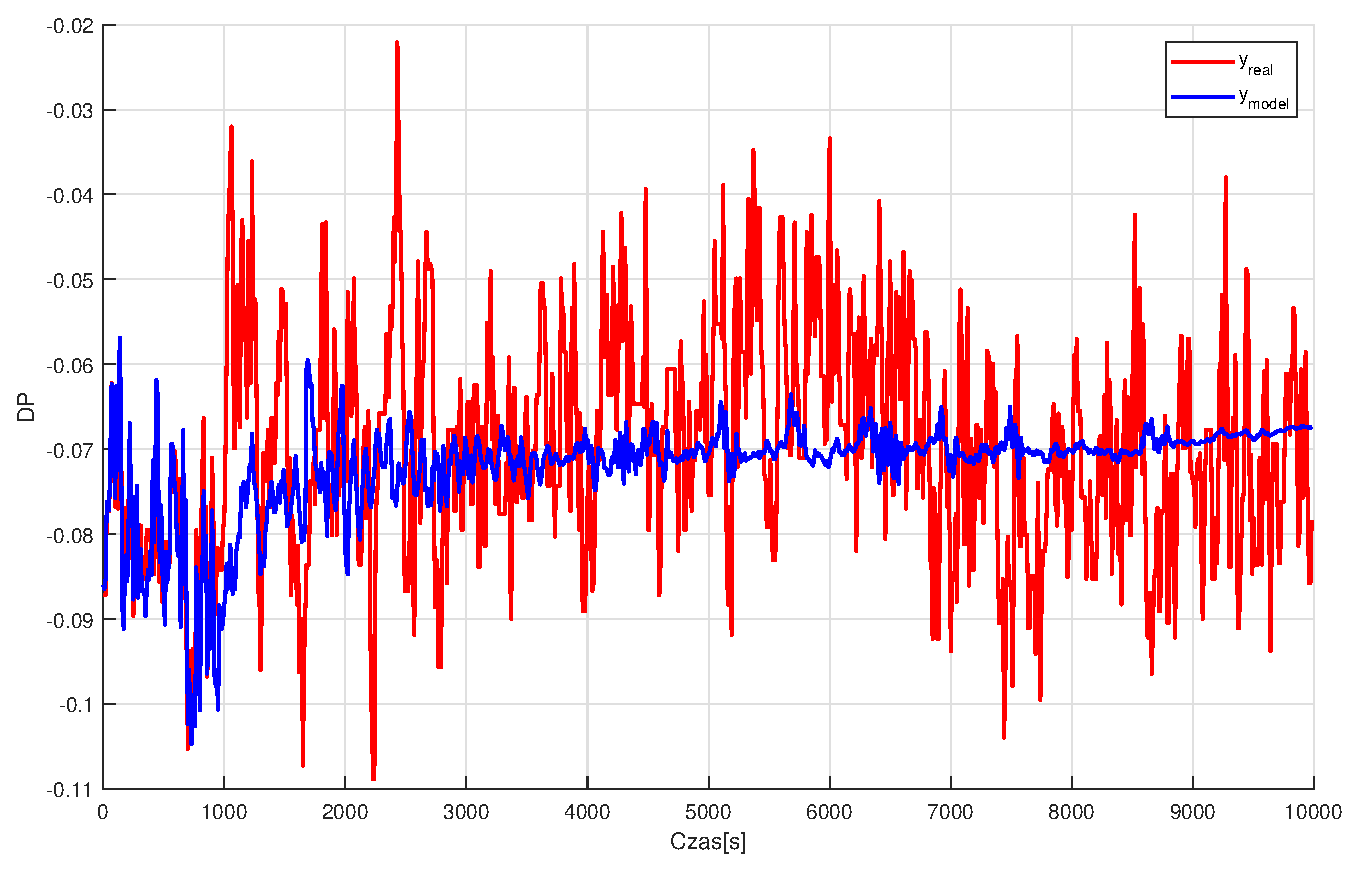
\includegraphics[width=0.75\linewidth,keepaspectratio]{results_matlab/DP_2.eps}
    \caption{Porównanie działania modelu ARX z danymi uczącymi (z. 2)}
    \label{fig:test}
    \end{figure}
\end{frame}

\addtocounter{framenumber}{-1}
\begin{frame}
  \frametitle{Działanie modelu ARX dla sygnału DP}
  \begin{figure}[H]
    \centering
    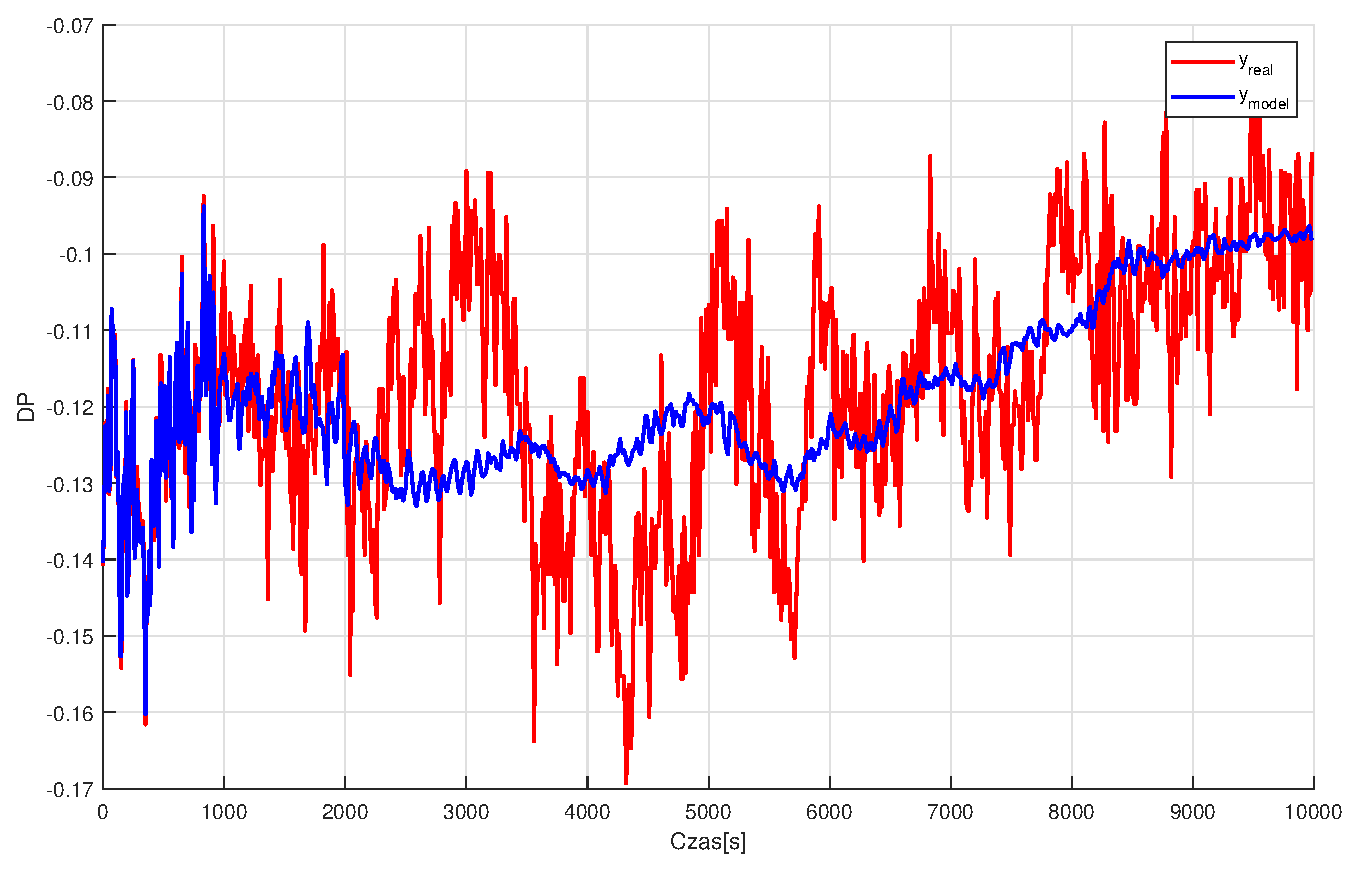
\includegraphics[width=0.75\linewidth,keepaspectratio]{results_matlab/DP_3.eps}
    \caption{Porównanie działania modelu ARX z danymi weryfikacyjnymi (z. 3)}
    \label{fig:test}
    \end{figure}
\end{frame}

\addtocounter{framenumber}{-1}
\begin{frame}
  \frametitle{Działanie modelu ARX dla sygnału DP}
  \begin{figure}[H]
    \centering
    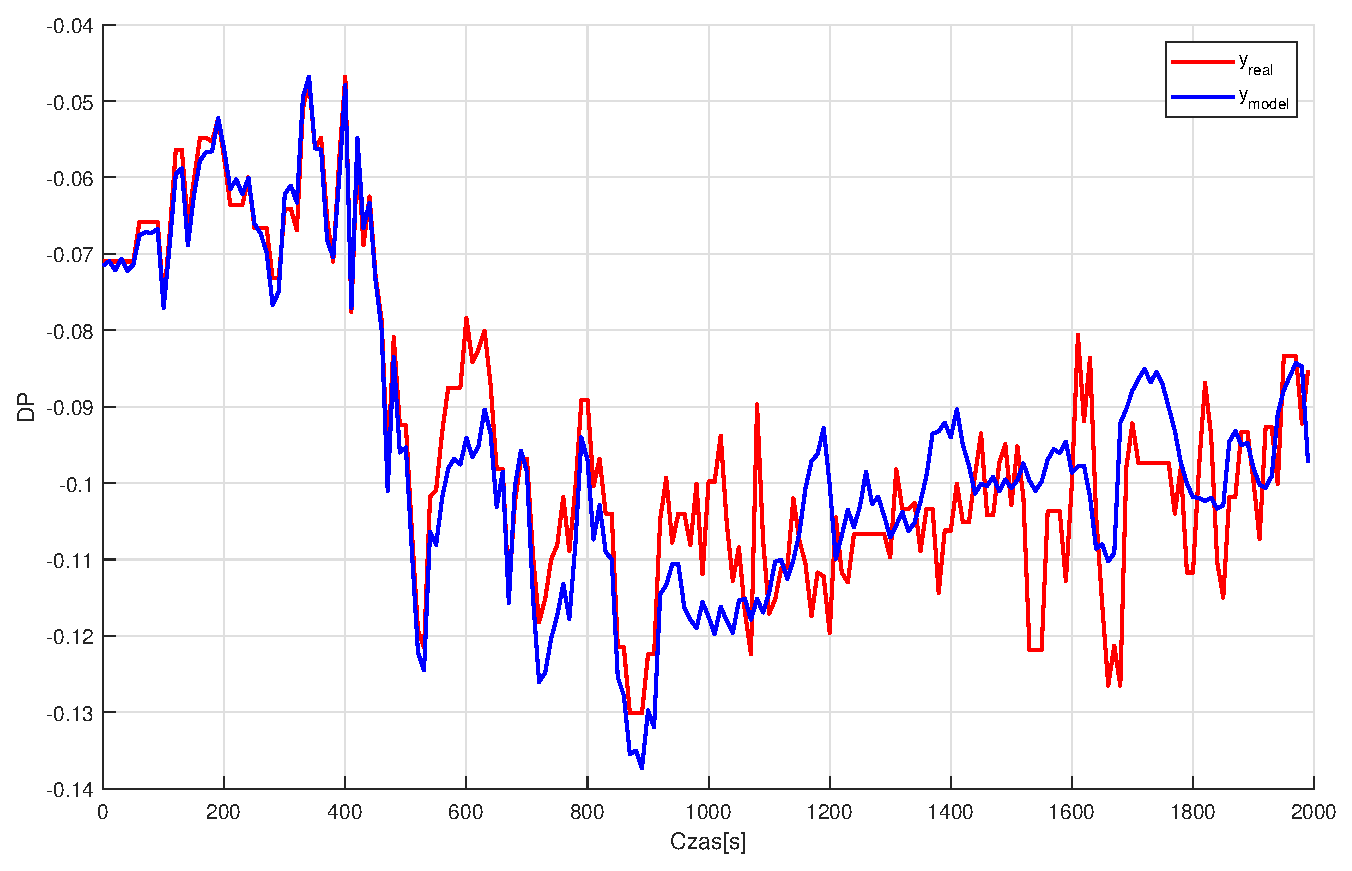
\includegraphics[width=0.75\linewidth,keepaspectratio]{results_matlab/DP_4.eps}
    \caption{Porównanie działania modelu ARX z danymi weryfikacyjnymi (z. 4)}
    \label{fig:test}
    \end{figure}
\end{frame}

\begin{frame}
  \frametitle{Model ARX - wady i zalety}
  \begin{exampleblock}{Zalety}
    \begin{itemize}
      \item łatwy do nauczenia,
      \item łatwo rozszerzalny.
    \end{itemize}
  \end{exampleblock}
  \begin{alertblock}{Wady}
    \begin{itemize}
      \item wysoki koszt obliczeniowy dopasowywania parametrów modelu ARX i minimalnej wartości współczynnika korelacji,
      \item do szukania parametrów wykorzystana MNK,
      \item złożoność rośnie nieliniowo względem wejść.
    \end{itemize}
  \end{alertblock}
\end{frame}